 \section{Scelte progettuali}
Durante il periodo di stage che ho sostenuto presso SAIV S.p.A., in
collaborazione con il tutor aziendale dott. Lovato Giovanni e il collega Rigoni
Giulio , è stata sviluppata un'applicazione per monitorare il livello di CS.

Questa applicazione è stata creata a seguito di una reale richiesta di una
commessa da parte di un'azienda. L'Ente aveva richiesto uno strumento intuitivo
e veloce da affiancare al ServQual, in modo da facilitare anche i clienti che
ritenevano troppo impegnativa la compilazione del questionario, coinvolgere
quindi quanti più utenti possibili, avere una maggiore quantità di dati ed un
feedback immediato.

Per diritti di privacy aziendale sostituirò il nome del committente con
l'Università degli Studi di Padova e ho adattato l'applicazione finalizzandola a
monitorare i servizi offerti dalla segreteria studenti.

\section{Presentazione del modello}

La nostra applicazione è certamente più veloce ed intuitiva rispetto al modello
ServQual.
Altro punto di forza dell'applicazione è l'automatizzazione. A differenza del
questionario cartaceo in cui poi risulta necessario registrare i dati,
elaborarli ed archiviarli, l'applicazione permette queste operazioni in tempi
veloci e contemporaneamente all'espressione del voto da parte del cliente, in
modalità automatica.

E' necessario evidenziare che il nostro modello non è esaustivo. E'
un'applicazione da affiancare ad altri strumenti, è una modalità che permette di
avere un feedback generale e veloce, ma non completo. Per essere un modello
valido sarebbe necessario elaborarlo ulteriormente.

L'utente ha la possibilità di esprimere la propria valutazione scegliendo tra le
possibilità: non del tutto soddisfatto, mediamente soddisfatto e molto
soddisfatto. Ad ogni alternativa abbiamo conferito un valore: a ``non del tutto
soddisfatto'' il valore 1, a ``mediamente soddisfatto'' il valore 3, a ``molto
soddisfatto'' il valore 5. La scelta dei valori è stata fatta per permettere, in
un tempo successivo, l'inserimento di altre valutazioni intermedie (2 e 4) che
faciliterebbero una visione più completa.

All'utente sarà permesso di esprimere il proprio voto in modo anonimo,
intuitivo e veloce con la possibilità di aggiungere un commento che verrà registra-
to dal sistema. L'amministratore, invece, potrà analizzare i dati, anche in tempo
reale, visualizzati su grafici. Ad una prima analisi della commessa con il team, è stata
presa la decisione di realizzare un' applicazione con una sezione front end, otti-
mizzata per eseguita su dispositivi touchscreen e una sezione back end accessibile
solo dagli amministratori.
Nel momento in cui ci siamo chiesti quali dati sarebbe stato utile salvare,
abbiamo deciso di registrare nel sistema il commento, il nominativo e l'e-mail
dell'utente (dati presentati come facoltativi, con il modello per la privacy e
l'utilizzazione dei dati), la data di votazione in formato gg/mm/aa, il
department per gli sportelli di facoltà e lo score. Il commento personale
permetterà all'ente di avere un riscontro più completo rispetto alla singola
risposta di scelta multipla e molto utile al fine di una verifica dei servizi
proposti, il nome e l'indirizzo di posta elettronica consentiranno al
committente di contattare la persona che lo ha richiesto e la data di votazione
può facilitare l'analisi dell'affluenza al servizio.

\section{Casi d'uso}
Inserimento della votazione, lato \emph{front end}:
\begin{itemize}
  \item \textbf{Voto in uscita} : In uscita dalla segreteria lo studente
  troverà un totem multimediale touch screen con cui potrà esprimere il
  proprio livello di soddisfazione dopo aver usufruito dei servizi offerti. La
  schermata di introduzione è composta da un messaggio inserito per spiegare
  all'utilizzatore la finalità per la quale viene richiesto di lasciare un
  \emph{feedback}, un video introduttivo dell'Università degli Studi di Padova
  e la scelta dell'operazione effettuata : servizio ricevuto presso lo sportello
  di facoltà o sportello veloce (Figura~\ref{fig:scorecard}).
  \item \textbf{Inserimento commento} : Lo studente può lasciare un proprio
  commento selezionando l'area con la voce ``Laciaci un commento''. Comparirà un finestra di dialogo che permetterà
  l'inserimento del testo , il nome e cognome e l'indirizzo email se il cliente
  vuole essere contattato. Per registrare il commento bisogna accettare le
  condizioni sulla privacy~(Figura~\ref{fig:comment}).
  \item \textbf{Registrazione del voto} : Il cliente esprime il proprio livello
  di soddisfazione tramite l’interfaccia selezionando uno dei 3 bottoni. In caso l'utente avesse
  selezionato nella schermata precedente la voce ``servizio sportello di
  facoltà'' un menu a tendina comparirà per indicare lo sportello difacoltà al
  quale si è rivolto~(Figura~\ref{fig:voting}).
  \item \textbf{Feedback all'utente} : Terminato il processo di registrazione
  una finestra di dialogo certifica all'utente che il processo di voto si è
  concluso in modo corretto~(Figura~\ref{fig:stored}).
    \begin{figure}[!h]
    \begin{center}
        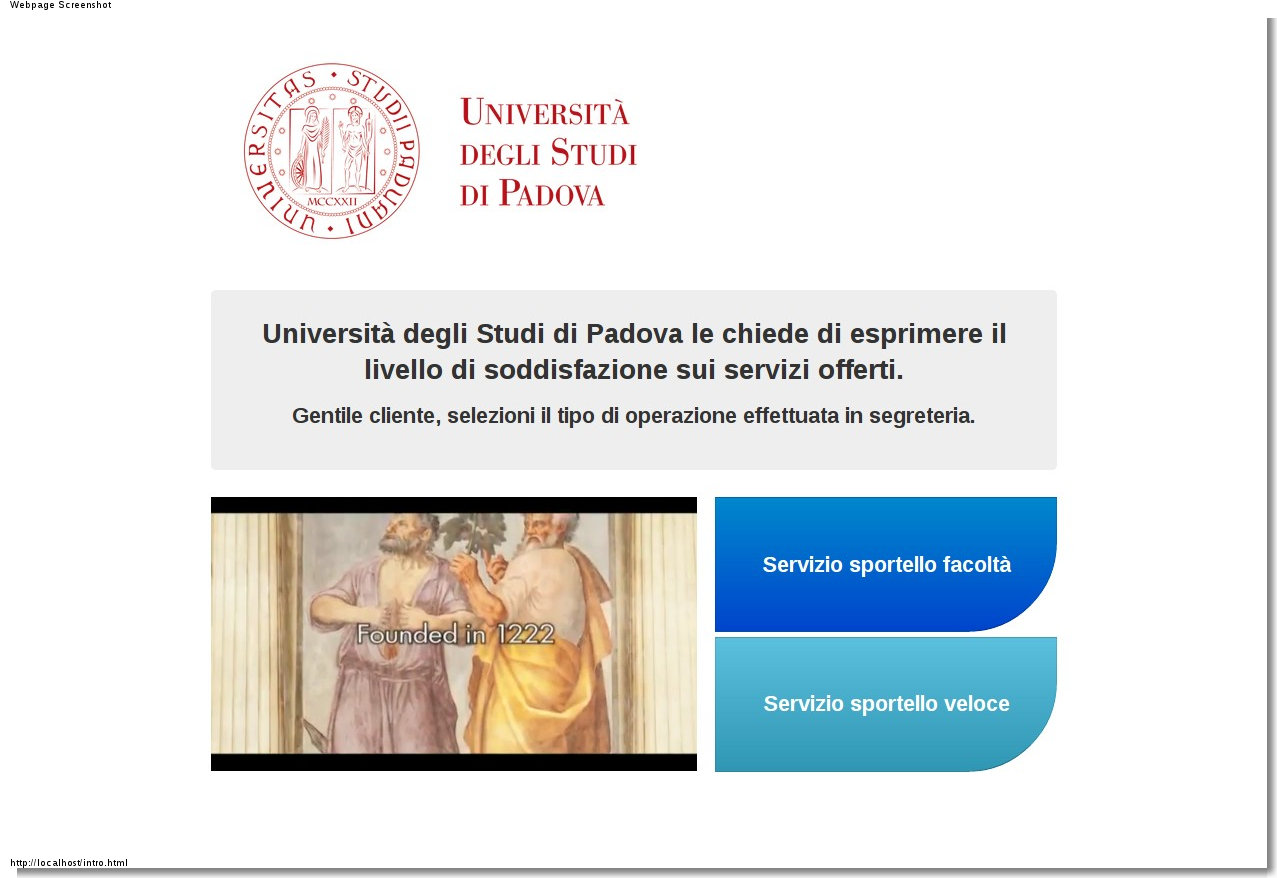
\includegraphics[scale=0.32]{scorecard.png}
        \caption{Schermata introduttiva}
        \label{fig:scorecard}
    \end{center}
  \end{figure}
   \begin{figure}[!h]
    \begin{center}
        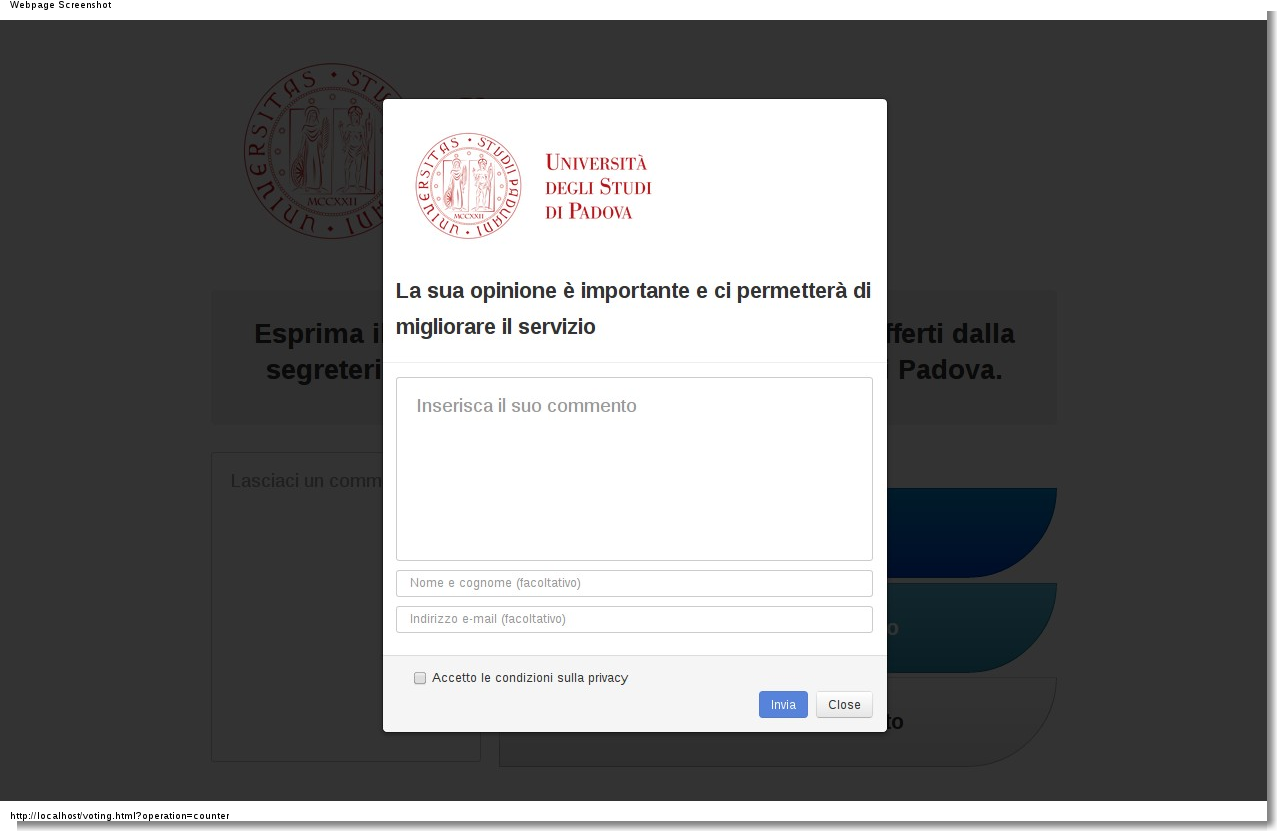
\includegraphics[scale=0.32]{comment.png}
        \caption{Inserimento di un commento}
        \label{fig:comment}
    \end{center}
  \end{figure}
   \begin{figure}[!h]
    \begin{center}
        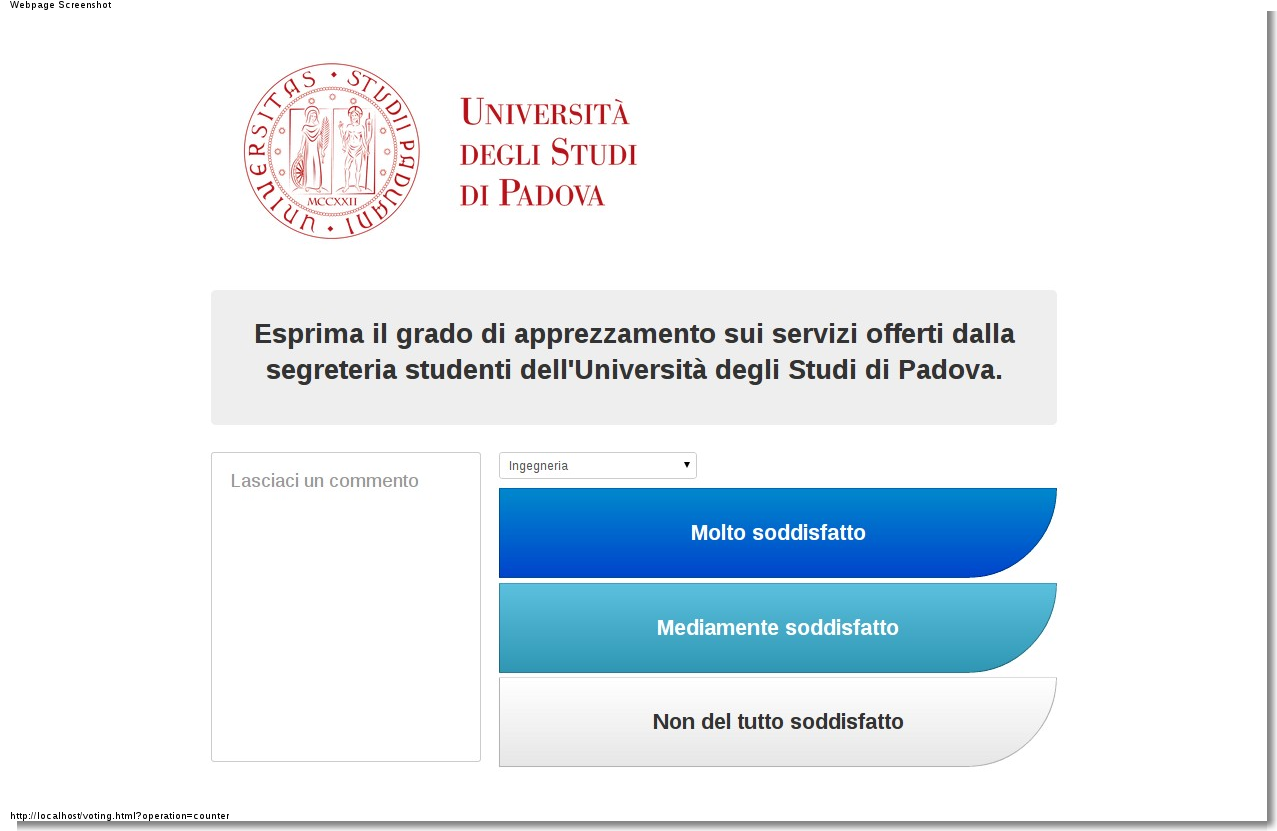
\includegraphics[scale=0.32]{voting.png}
        \caption{Scelta del livello di soddisfazione}
        \label{fig:voting}
    \end{center}
  \end{figure}
  \begin{figure}[!h]
    \begin{center}
        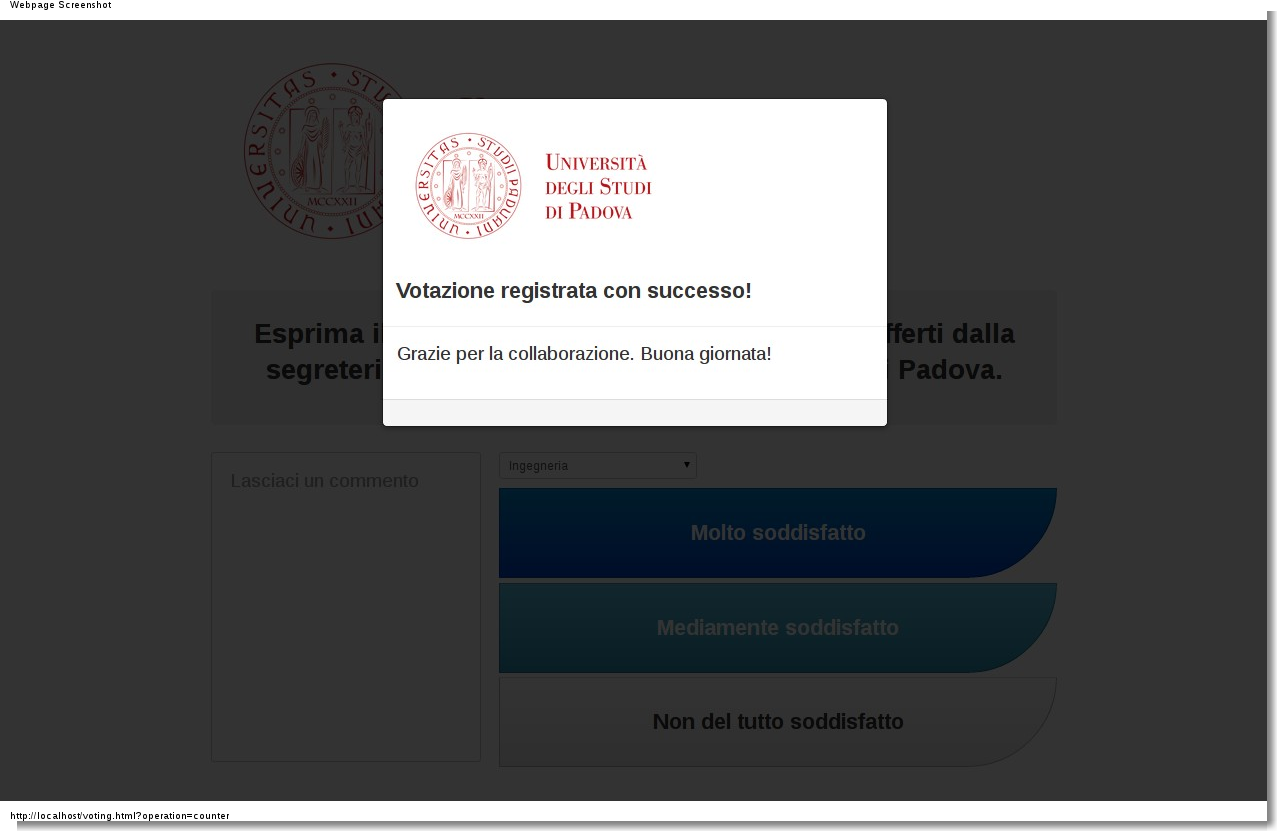
\includegraphics[scale=0.32]{stored.png}
        \caption{Feedback all'utente}
        \label{fig:stored}
    \end{center}
  \end{figure}
\end{itemize}
\\\\
Consultazione dei voti \emph{back end}:Caso d’uso 2 (Consultazione dei voti). Un altro caso d’uso prevede la consultazione dell’andamento del livello di CS da parte
dell’Amministratore del Sistema (vedi Figura 2). L’Amministratore del Sistema potrà accedere via browser web a un’interfaccia
di consultazione dei voti, che presenterà in modo grafico l’andamento del livello di CS filiale per filiale.
1. L’Amministratore accede all’interfaccia web del Sistema.
2. Il Sistema genera i grafici relativi all’andamento della CS

\section{Classi}

\section{Strumentazione}
I linguaggi in cui verrà sviluppato il sistema sono HyperText Markup Language (HTML), Cascading Style Sheets (CSS) e
JavaScript (JS) con database di appoggio CouchDB, tramite i quali sarà implementata un’applicazione web aderendo al paradigma Model-View-Controller (MVC).